\documentclass{article}
\usepackage[utf8]{inputenc}
\usepackage{minted}
\usepackage{listings}
\usepackage{hyperref}
\usepackage{graphicx}
\graphicspath{ {screenshots/} }

\title{ SR Peru Code Documentation}
\author{ Brett Fox and Jared Olson }
\date{ July 2018 }

\begin{document}

\maketitle

\newpage
\tableofcontents
\newpage

\section{Adding A New Model}
We have split the models out so each section of the page (Participant, Entomology, FSS\_FLU) has its own \textit{.py} file located in \textit{form\_manager/models/}.  Each model is then being imported into the \textit{form\_manager/models/\_\_init\_\_.py} file so that in any other file when you want to import a model you can do so with:
\begin{minted}{python}
from form_manager.models import model_name
\end{minted}
\subsection{Model File Definitions}
\textbf{entomology\_models.py:} Contains model definitions for the Entomology section of the website including any option models that the Entomology models reference.

\textbf{fss\_flu\_models.py:} Contains model definitions for the FSS-FLU section of the website (Cohort and Clinic forms) including any option models that the FSS-FLU models reference.

\textbf{gis\_models.py:} Contains model definitions for the GIS and Location models.  Django does not and should not manage these tables.  They reside in a different Postgres schema and are being managed separately.

\textbf{participants\_models.py:} Contains model definitions for the Participant section of the website including any option models that the Participant models reference. It also includes Adverse Event models.

\textbf{reference\_models.py:} Contains model definitions for Reference tables and any option models that the Reference table models reference.  It also includes the Form Note model and Language Preference Model that we are using to extend the User model.

\subsection{UUID Primary Key and Many-To-Many Tables}
\subsubsection{UUID Primary Key}
To prevent collisions of primary keys when the UC Davis server syncs with the two servers in Peru we are changing the primary key of each model from the auto-incremented integer that Django provides to a UUID field. This involves defining the id field manually in the model like so:
\begin{minted}{python}
    id = models.UUIDField(primary_key=True, default=uuid.uuid4, 
    editable=False)
\end{minted}
\subsubsection{Many-To-Many Tables}
Normally, for many-to-many relationships Django will automatically create and manage an intermediate table. However, it does allow users the ability to manually manage an intermediate table. We manually define all many-to-many intermediate tables so we can change the ID field to a UUID field. Information regarding this process can be found in the resources section.
\\We have a custom function for saving many-to-many relationships in views. It is located in \textit{form\_manager/helpers/save\_custom\_m2m()}. This function requires that the form which contains the many-to-many relationship you are trying to save has an a proper entry in the \textit{global\_variables.py} file like so:
\begin{minted}{python}
'many-to-many_definitions': [
    {
        'model': ParticipantFormCensusForm,
        'form_field_name': 'census_id',
        'field_name_1': 'participant_form',
        'field_name_2': 'census_form',
    },
]
\end{minted}

\textbf{model}: The many-to-many model name

\textbf{form\_field\_name}: The name of the field in the original form model.

\textbf{field\_name\_1}: The name of the foreign-key field in the many-to-many table that links to the form model.

\textbf{field\_name\_2}: The name of the foreign-key field in the many-to-many table that links to the other model.

\subsection{Migrations}
Due to constraints on the UC Davis server the migrations must always be squashed to only include the initial migration.  This means that after model changes are made, all migrations must be deleted before running:
\begin{lstlisting}[language=bash]
  python manage.py makemigrations
\end{lstlisting}

\section{Adding A New Form}
The form definitions reside in \textit{form\_manager/forms/} and are split into individual files for each page section (Participant, Entomology, FSS\_FLU). 
\\\\We are taking advantage of Django's built in \textit{ModelForm} class to define forms. This class requires you to have a model already created for the form you are implementing.
\\\\Any custom form validation is being handled in these form classes via the \textit{clean()} method.
\\\\The order of the fields displayed on the front end is being assigned in the \textit{get\_context\_data()} method in whichever Create/Update view is handling the current form.  They are being handled in the context variable \textit{field\_rows}.  For example:
\begin{minted}{python}
context['field_rows'] = [
    [form['family']],
    [form['first_name'], form['last_name'], form['last_name2']],
    [form['sex'], form['birthdate']],
    [form['neighborhood_years'], form['neighborhood_months']],
    [form['house_years'], form['house_months']],
    [form['history']],
    [form['fs_age'], form['fs_address'], form['fs_weight']],
    [form['review']],
    [form['comments']],
]
\end{minted}

\section{Adding a New List View}
The list tables on the site are using a jQuery plugin called DataTables.  DataTables expects a dictionary object that it can manipulate on the front end, but this causes problems with extremely large data sets like those we are working with. To solve this, we are handling all of the sorting, searching, and pagination ourselves by taking advantage of DataTables' ability to allow server side processing. 
The advantage of this is that we can pass a dictionary of the 10-100 items needed to be displayed instead of the entire data set, which could be upwards of 250,000 items.
\\\\The DataTable is empty to begin with and a request is being sent via AJAX that passes the table parameters (search values, page number, sorted column, etc.) to a function that uses this information to gather a dictionary of items the table should display. 
\\\\In order for our DataTables function to work correctly we must create an entry in our global variable dictionary located in \textit{form\_manager/global\_variables.py}.  This global variables dictionary allows for code to be dynamic.  It is used throughout our code but it is critical to add any new form you want displayed in a list or detail page to the dictionary.  Below is an example of a global variable entry:
\begin{minted}{javascript}
'participant': {
        'model': ParticipantForm,
        'active': 'participant_detail',
        'form_class': ParticipantFormForm,
        'breadcrumb_name': 'Participant Detail',
        'id_title': 'Participant ID',
        'searches': {
            'Participant ID': ['id'],
            'First Name': ['first_name'],
            'Last Name': ['last_name'],
            'Last Name2': ['last_name2'],
            'Birthdate': ['birthdate'],
            'Family': ['family'],
            'Neighborhood Years': ['neighborhood_years'],
            'Neighborhood Months': ['neighborhood_months'],
            'House Years': ['house_years'],
            'House Months': ['house_months'],
            'History': ['history'],
            'FS Age': ['fs_age'],
            'FS adminAddress': ['fs_address'],
            'Review': ['review'],
            'Comments': ['comments'],
            'FS Weight': ['fs_weight'],
            'Sex': ['sex__option'],
            'Censuses': ['census_id__project__project_code', 'census_id__location__location_code', 'census_id__id'],
            'Entered By': ['entered_by__username'],
            'Entered Date': ['entered_date'],
            'Updated Date': ['updated_date'],
            'Updated By': ['updated_by__username'],
            'Participant Codes': ['participant_participantCode__participant_code'],
            'Studies': ['participant_consent__study__study'],
            'Age': None
        },
        'many_to_many_fields': {
            'Participant Codes': 'participant_participantCode__participant_code',
            'census_id': 'census_id__id',
            'Studies': 'participant_consent__study__study'
        },
        'order': [
            'id', 'Participant Codes', 'census_id', 'Studies', 'family', 'first_name', 'last_name', 'last_name2',
            'sex', 'birthdate', 'Age', 'neighborhood_years', 'neighborhood_months', 'house_years', 'house_months',
            'comments', 'history', 'fs_age', 'fs_weight', 'fs_address', 'review', 'entered_by', 'entered_date',
            'updated_by', 'updated_date',
        ],
        'incomplete_searchable_fields': ['Participant ID', 'Censuses', 'Participant Codes', 'First Name', 'Last Name',
                                         'Last Name2', 'Entered By', 'Updated By'],
        'many-to-many_definitions': [
            {
                'model': ParticipantFormCensusForm,
                'form_field_name': 'census_id',
                'field_name_1': 'participant_form',
                'field_name_2': 'census_form',
            },
        ]
    }
\end{minted}
The most important fields for this feature are outlined below:

\textbf{searches}: Any fields you are allowing to be searched must be added to this dictionary. The key must be the field as displayed on the front end after titling has been applied. The value must be a list of the actual model fields used to search the field when using the Django ORM. That value will be literally placed into a query string when used. It is a list because there are instances where multiple fields must be queried.

\textbf{many\_to\_many\_fields}: Many-to-many relationships are handled differently than other field types, so their search fields are defined in a separate dictionary. If the field is a model field then the key must be the literal field name. Otherwise, the key must be the field as displayed on the front end after titling has been applied. In either case, the value must be the actual model field used to search the field when using the Django ORM.

\textbf{order}: This list will be used to determined the field order of both the list and detail pages.  Each field must be in the format it is given in the model.  The exception to this are fields added that don't exist within the model. Those must be fields as displayed on the front end after titling has been applied.

\section{Adding a New Model Field}
When adding a new field to an existing form model then you would need to refer to sections 1-3 to get the field to display correctly on the website.

\section{Adding Field Options}
Only users with the permission, '\textit{Reference Table Admin}, are able to add new drop-down options and Reference table entries.  They will do so by accessing the Admin page.  The Admin page has been filtered to show only tables they can edit. For example, form tables are not available for them to edit in the Admin page. The Admin page is grouped by model type (Reference Table, Participant, Entomology, FSS-Flu, Shared Tables). The forms that use the Option model are also listed. 
\\
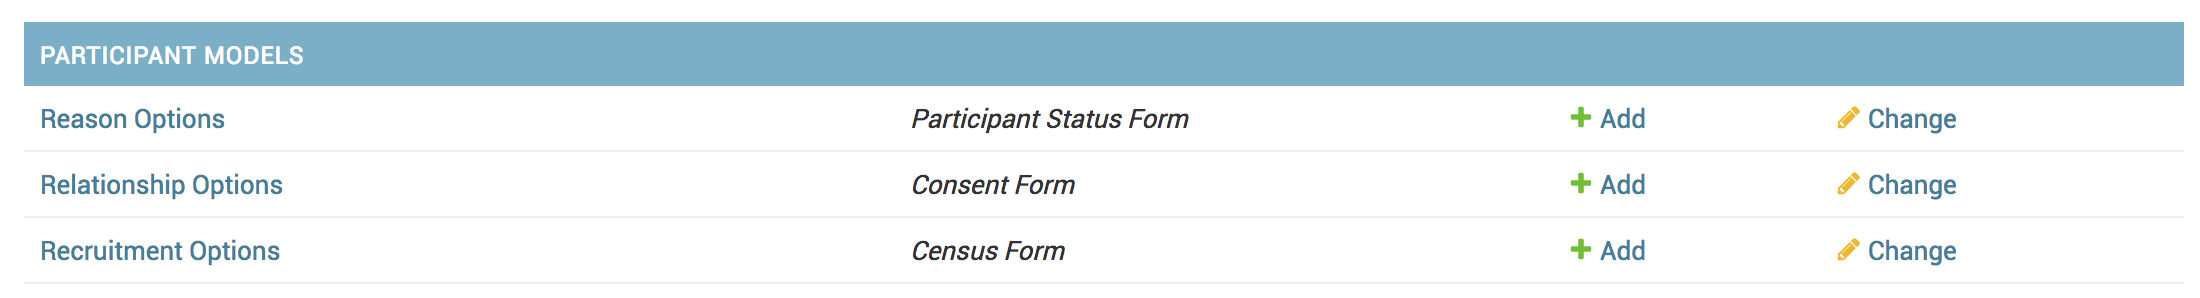
\includegraphics[width=\textwidth,height=\textheight,keepaspectratio]{/admin_screenshot}
\section{Fixtures}
There is a custom management script that will load all of the necessary fixture files:
\begin{lstlisting}[language=bash]
  python manage.py load_fixtures
\end{lstlisting}
The fixture files are defined below:

\textbf{auth\_group.json}: Handles definitions of auth\_group tables, mainly to define which tables will appear editable for Reference Table Admins.

\textbf{auth\_users.json}: Handles definitions of auth\_user tables. These are people that may log into the site and their permissions.

\textbf{options.json}: Handles definitions of any 'Option' tables.  'Option' tables include those tables that only hold drop-down option choices. e.g. YesNoOption, ResidentialOption, ComplaintOption.

\textbf{r\_tables.json}: Handles definitions of 'Reference' tables.  Reference tables are drop-down choices but also hold more critical information.  e.g. Personnel, Project, Study.

\section{Translation Overview}
The built in Django User table is being extended to include a \textit{language\_preference} field so each user of the site's language preference can be saved whenever they switch languages on the site. This is happening in \textit{reference\_models.py}.
\\\\There is a \textit{change\_language} function in \textit{form\_manager/views/translations.py} that is called anytime the change language button is clicked on the site.  It sets that user's language preference to the newly selected language.  This only sets the user's preferred language
\\\\There is a middleware function, located in \textit{form\_manager/middleware.py}, which runs with every request that actually tells the backend which language to use.

\section{Adding/Updating Translations}
Translations are handled in \textit{locale/es/LC\_MESSAGES/django.po} for English to Spanish and \textit{locale/en/LC\_MESSAGES/django.po} for Spanish to English. 
\\\\After adding or updating the translation in the English to Spanish \textit{django.po} file, run the following command for the changes to take effect:
\begin{lstlisting}[language=bash]
  python manage.py compilemessages
\end{lstlisting}
Then run the following script which updates the Spanish to English \textit{django.po} file automatically:
\begin{lstlisting}[language=bash]
  python manage.py make_english_po
\end{lstlisting}

\section{Dropdown Sorting}
Most dropdown options on the website are being ordered alphabetically. But this is quite difficult to do on the backend when dealing with translations, so we are sorting them via JavaScript in the file \textit{static/js/sort\_dropdown.js}.
\\\\Any dropdown options you don't want to sort alphabetically on the front end must be added to the 'dropdowns\_to\_ignore' list in the same JavaScript file.

\section{Admin Customization}
Admin templates exist in the path \textit{form\_manager/templates/admin/} so they can be overwritten.  It is important not to change the structure of the files or remove these templates. We are overwriting form\_manager templates to include a new JavaScript file which will change the form widgets for 'Location' fields on the admin page. The \textit{base.html} and \textit{index.html} are being overwritten to customize table grouping on the main admin page.
\\\\
The \textit{AdminSite} class is being instantiated so we can add data to pass to the \textit{index.html} template.  This is how we are customizing the main Admin page. This is happening in \textit{form\_manager/admin.py}. Inside this class, \textit{MyAdminSite}, we are accessing a global variables file that defines what tables should be grouped where. This is defined in \textit{form\_manager/admin\_global\_variables.py}.

\section{ETL Script}
The ETL is split into two different scripts.
\\\textit{form\_manager/management/commands/run\_callao\_etl.py} is the ETL script for all Entomology tables.  \\\textit{form\_manager/management/commands/run\_participant\_etl.py} is the ETL script for all Participant and FSS\_FLU tables. The scripts can be worked on and run independently because they grab their data from completely different tables. They reside in the commands folder so they can be run as django management commands using:
\begin{lstlisting}[language=bash]
  python manage.py run_callao_etl
  python manage.py run_participant_etl
\end{lstlisting}
The models they reference reside in \textit{form\_manager/ETL\_Script/PD\_models.py}.  The helpers file in the same path holds mapping definitions for the ETL scripts.

\section{Template Naming Structure}
The project has a naming convention for HTML files to help organize types of templates.  HTML files with an underscore before the name, such as \textit{\_footer.html}, are templates that will be included in other HTML files.

\section{Resources}
\textbf{Datatables:} \url{https://datatables.net/manual/}
\\\textbf{Datatables Server Side Processing:} \url{https://datatables.net/manual/server-side}
\\\textbf{Django Translation:} \url{https://docs.djangoproject.com/en/2.0/topics/i18n/translation/}
\\\textbf{Bootstrap Select:} \url{https://silviomoreto.github.io/bootstrap-select/}
\\\textbf{Manually Handling Intermediate Tables in Django: }\url{https://docs.djangoproject.com/en/1.11/topics/db/models/}
\end{document}
